%! TEX root = main.tex

%/========== Variable Length Pendulum ==========/%
\chapter{Application of VNHCS: The Variable Length Pendulum}\label{sec:vlp}
\section{Motivation}
The variable length pendulum (VLP) is a classical underactuated dynamical system
which is often used to model the motion of a person on a swing
\cite{pumping_swing_standing_squatting,how_to_pump_a_swing}.
The VLP also represents the swinging of a crane, the (simplified) motion of a
gymnast on a bar \cite{pendulum_length_giant_gymnastics}, and the
tuned-mass-damper systems which stabilize skyscrapers
\cite{vlp_tuned_mass_damper}.

The motion of the VLP has been well studied (see for instance
\cite{dynamics_periodic_vlp}), and many control mechanisms exist
to stabilize trajectories of the system. While many of these controllers 
are time-dependent, \cite{vlp_energy_shaping}
offers a time-independent technique to inject energy into the system and
stabilize desired energy level sets. The authors designed a controller through a
technique called \textit{energy shaping}, and proved that their control
mechanism would allow the VLP to achieve any desired energy level set.
However, the energy injection mechanism is
ad-hoc in the sense that it is not derived from natural behaviour. In
this chapter we will design VNHCs to inject energy into the VLP in a
time-independent way.
The difference compared to \cite{vlp_energy_shaping} is that our 
controller will maintain the structured motion of a human on a swing.

\section{Dynamics of the Variable Length Pendulum}
% Derive the dynamics of the VLP in Hamiltonian form
We will model the VLP as a point mass \(m\)
connected to a fixed pivot by a massless rod of varying length \(l\) with angle 
\(q \in \mathbb{S}^1\) from the vertical, as is seen in Figure
\ref{fig:vlp-model}. 
We will also ignore any damping and frictional forces in this model.
In a realistic VLP, the rod length \(l\) varies between some minimum
length \(\underline{l} \geq 0\) and some maximum length 
\(\overline{l} > \underline{l}\). The configuration of the VLP is the vector
\(\mathbf{q} := (q,l) \in \mathbb{S}^1 \times [\underline{l},\overline{l}]\).

\begin{figure}
   \centering
   \includestandalone[width=0.5\textwidth]{images/vlp_model}
   \caption{The representation of the variable length pendulum as a mass at the
      tip of a massless rod.}\label{fig:vlp-model}
\end{figure}

Using this configuration, we will compute the Hamiltonian dynamics of the system.
The cartesian position of the mass at the tip of the pendulum
is given by \(x = (l\sin(q),l\cos(q))\), while its velocity is
\(\dot{x} = (\dot{l}\sin(q) + l\cos{q}\dot{q}, \dot{l}\cos(q) - l\sin{q}\dot{q})\).
Computing the kinetic energy \(T\) yields
\[
   T(\mathbf{q},\dot{\mathbf{q}}) = 
   \frac{1}{2}m\norm{\dot{x}}^2 = \frac{1}{2}m\left(\dot{l}^2 + l^2\dot{q}^2\right)
\]
The potential energy \(P\) with respect to the pivot (under a gravitational
acceleration \(g\)) is
\[
   P(\mathbf{q}) = -mgl\cos(q)
\]
Collecting the kinetic energy into a quadratic form, we get the Lagrangian
\[
   \mathcal{L}(\mathbf{q},\dot{\mathbf{q}}) 
   = \frac{1}{2} \dot{\mathbf{q}}\tpose D(\mathbf{q})\dot{\mathbf{q}} - P(\mathbf{q})
   = \frac{1}{2}
   \begin{bmatrix} \dot{q} & \dot{l} \end{bmatrix}
   \begin{bmatrix}
      ml^2 & 0 \\
      0 & m \\
   \end{bmatrix}
   \begin{bmatrix} 
      \dot{q} \\ \dot{l}
   \end{bmatrix}
   + mgl\cos(q)
\]
Computing the conjugate of momenta to \(\mathbf{q}\), we get 
\[
   \mathbf{p} := \begin{bmatrix} p \\ p_l \end{bmatrix} 
   = \begin{bmatrix} ml^2\dot{q} \\ m\dot{l} \end{bmatrix} 
\]
Performing the Legendre transform on \(\mathcal{L}\) and setting
\(M(\mathbf{q}) := D(\mathbf{q})\), \(V(\mathbf{q}) := P(\mathbf{q})\),
we find the Hamiltonian is equal to the total mechanical energy of the system:
\[
   \mathcal{H} = E = \frac{1}{2}\dot{\mathbf{p}}\tpose \Minv(\mathbf{q})
   \dot{\mathbf{p}}+V(\mathbf{q})
\]
Taking the appropriate derivatives, the dynamics of the VLP in Hamiltonian form
are described in (\ref{eqn:vlp-hamiltonian-with-pl}). 
\begin{align}\label{eqn:vlp-hamiltonian-with-pl}
   \mathcal{H} &= \frac{1}{2} \begin{bmatrix} p & p_l \end{bmatrix}
      \begin{bmatrix}
         \frac{1}{ml^2}  & 0 \\
         0 & \frac{1}{m}
      \end{bmatrix} \begin{bmatrix} p \\ p_l \end{bmatrix} - mgl\cos(q) \\
     &\begin{cases}
        \dot{q} = \frac{p}{ml^2} \\
        \dot{l} = \frac{p_l}{m} \\
        \dot{p} = -mgl\sin(q) \\
        \dot{p}_l = \frac{p^2}{ml^3} + mg\cos(q) + \tau \\
   \end{cases} \nonumber
\end{align}
The control input is a force \(\tau \in \mathbb{R}\) affecting the dynamics of
\(p_l\), acting colinearly with direction of the rod.
We assume the force does not affect the dynamics of \(p\) in any way -
that is, the control input cannot enact any lateral force on the pendulum.
This is extremely useful for simplifying the dynamics: since one can choose
\(\tau\) which sets \(\dot{p}_l\) to any desired function, we can assume (with abuse
of notation) that \(l\) is tracking some known function \(l(t)\). 
The closed loop dynamics of the system will be described exclusively by
\((\dot{q},\dot{p})\) with \(l \equiv l(t)\).
The fact that \(p_l\) does not appear in these closed-loop dynamics allows us to
ignore the subdynamics \((\dot{l},\dot{p}_l)\) entirely. 

What this means is we can treat \(l\) as the control input directly, rather than
modelling it as a configuration variable. Re-deriving the Hamiltonian and the
dynamics from this approach, we get the system 
(\ref{eqn:vlp-hamiltonian}) with phase \((q,p) \in \mathbb{S}^1 \times \R\). 
Note that the control input \(l(t)\) and its derivative \(\dot{l}(t)\) are both
known variables.
\begin{align}\label{eqn:vlp-hamiltonian}
   \mathcal{H}(q,p) &= \frac{p^2}{ml^2} - \frac{1}{2}\dot{l}^2 - mgl\cos(q) \\
     &\begin{cases}
        \dot{q} = \frac{p}{ml^2} \\
        \dot{p} = -mgl\sin(q) \\
      \end{cases}\nonumber
\end{align}
In particular, the Hamiltonian of this simplified model is no longer equal to
the total mechanical energy of the system, which is given by
(\ref{eqn:vlp-energy}).
\begin{equation}\label{eqn:vlp-energy}
   E(q,p) = \frac{p^2}{ml^2} + \frac{1}{2}\dot{l}^2 - mgl\cos(q)
\end{equation}

% TODO: Describe the oscillation and rotation motion of a pendulum in the
% qp-plane, and give a figure showing the orbiting motion for each of these.
% Then describe what the orbit should do under energy injection (spiral away /
% begin rotation outward) and energy dissipation (spiral in / rotate inward).

\section{The VLP Constraint}
% TODO: Go through the development of the constraint and prove it gains energy
% TODO: Explain how we came up with the constraint first. Talk about the child
% on a swing, the paper showing the time-optimal control input, and describe why
% we want to remove time from the equation. Discuss the lmin and lmax choices.
% Why do we need to use a VNHC instead of a VHC: we are modelling the
% time-optimal controller in a time-independent way, which requires knowledge of
% which quadrant in (q,p)-space we're in. This means using the angle theta,
% which is inherently a VNHC.
Since we wish to define a VNHC which injects energy into the VLP in a human-like
manner,
we return once again to the example of a person standing on a swing.
As can be seen in Figure \ref{fig:child-vlp}, condensing the person 
into a center of mass gives a VLP model of their motion, where
the pendulum shrinks when the person stands and lengthens when they squat. This
is equivalent to the VLP model from Figure \ref{fig:vlp-model}.
\begin{figure}
   \centering
   \begin{subfigure}[t]{0.45\textwidth}
      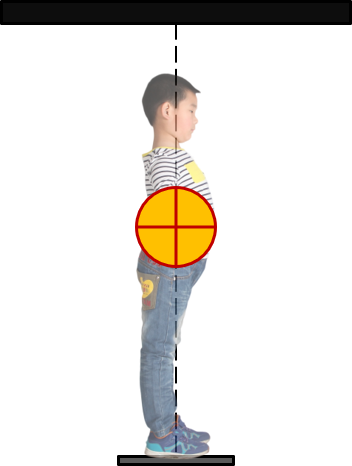
\includegraphics[]{images/child_vlp_standing.png}
      \caption{A person standing on a swing has their center of mass 
      close to the pivot.}
   \end{subfigure}
   \hfill
   \begin{subfigure}[t]{0.45\textwidth}
      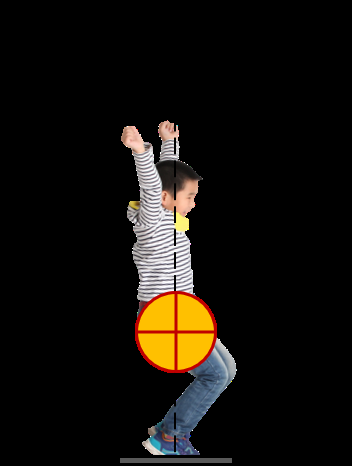
\includegraphics[]{images/child_vlp_squatting.png}
      \caption{When a person squats on a swing, their center of mass extends
      away from the pivot.}
   \end{subfigure}
   \caption{The variable length pendulum representation of a person on a
   standing swing.}\label{fig:child-vlp}
\end{figure}

The action of regulating pendulum length to add energy to the VLP is known as
``pumping". \citeauthor{pumping_swing_standing_squatting} asked whether
the pumping strategy performed by children is time-optimal, assuming the
children could squat or stand instantaneously
\cite{pumping_swing_standing_squatting}. Indeed, they discovered that 
a child's pumping strategy will inject energy into the VLP as fast as is 
physically possible. 

This pumping strategy is straightforward: the child stands up at the lowest point of
their swing, and squats at the highest point. Looking at their VLP
representation, the pendulum shortens at the bottom of the swing, and lengthens
at the top. For an intuitive understanding, conservation of angular momentum
indicates that shortening the pendulum at the bottom forces the mass to gain
speed to compensate for the reduced length
\cite{how_to_pump_a_swing}.
Energy is not conserved in this process, and the pendulum gains kinetic energy
which allows the pendulum to reach a higher point in its swing.
Lengthening the pendulum when it reaches this point means gravity
imparts a larger angular momentum to the mass by the time it reaches the bottom
of its swing, which is converted into a higher velocity the next time the
pendulum is shortened.
By alternating these processes, the pendulum experiences a net gain in
rotational energy which is generated entirely by gravity.

The time-optimal controller described by \cite{pumping_swing_standing_squatting}
depends on a trajectory in time. We will convert this 
into a time-independent controller derived from the time-optimal
strategy. Notice that the optimal controller depends on knowing when the
system is at the ``bottom" or ``top" of the swing. Since being at the ``bottom"
is the same as saying the pendulum angle is \(q = 0\) and being at the ``top" is
equivalent to the pendulum's momentum being \(p = 0\), the time-independent
controller will necessarily use the full phase \((q,p)\). While VHCs cannot
satisfy this requirement, our method of VNHCs is especially well suited to this
problem.

Figure \ref{fig:vlp-optimal-controller-qp-plane} shows the time-optimal strategy directly
on the \((q,p)\)-plane.
Since the VLP must stay the same length inside each quadrant and
changes length only when it crosses one of the axes, we
will use the angle \(\theta = \arctan_2(p,q)\) in the \((q,p)\)-plane to define
the optimal controller \(l^\star(\theta)\) (\ref{eqn:vlp-optimal-controller}).
Figure \ref{fig:vlp-optimal-controller} shows this time-optimal controller as a function of
\(\theta\).
\begin{equation}\label{eqn:vlp-optimal-controller}
   l^\star(\theta):= \begin{cases}
      \underline{l} & \theta \in [-pi, -\frac{\pi}{2}[ \cup [0,\frac{\pi}{2}[ \\
      \overline{l} & \theta \in [-\frac{\pi}{2},0[ \cup [\frac{\pi}{2}, \pi[ \\
   \end{cases}
\end{equation}

\begin{figure}
   \centering
   \includestandalone[width=0.5\textwidth]{images/vlp_optimal_controller_qp_plane}
   \caption{The representation of the time-optimal controller for a standing
      swing in the \((q,p)\)-plane. As per 
      \cite{pumping_swing_standing_squatting}, the red region corresponds to
      squatting and the blue region corresponds to standing.}
      \label{fig:vlp-optimal-controller-qp-plane}
\end{figure}

\begin{figure}
   \centering
   \includestandalone[width=0.5\textwidth]{images/vlp_optimal_controller}
   \caption{The time-optimal VLP controller converted to a discontinuous
   function \(l(\theta)\), where \(\theta := \arctan_2(p,q)\).}\label{fig:vlp-optimal-controller}
\end{figure}

To find a continuously differentiable function which approximates this controller,
we can attach sinusoids at the transition points of
\(l^\star(\theta)\) (see Figure \ref{fig:vlp-T-controller}). Let
\(\Delta l := (\overline{l} - \underline{l})/2\) and 
\(l_{\text{avg}} := (\overline{l} + \underline{l})/2\).
Providing these newly attached sinusoids with a frequency \(\omega = \frac{pi}{T}\) 
(where \(T \in ]0,\frac{\pi}{2}]\) is a control parameter), we have a new
controller \(l_T(\theta)\):
\begin{equation}\label{eqn:vlp-T-controller}
   l_T(\theta) = \begin{cases}
      \underline{l} & \theta \in \left[-\pi + \frac{T}{2}, -\frac{\pi}{2} - \frac{T}{2}\right] 
      \cup \left[\frac{T}{2}, \frac{\pi}{2} - \frac{T}{2}\right] \\
      \overline{l} & \theta \in \left[-\frac{\pi}{2} + \frac{T}{2}, -\frac{T}{2}\right] 
      \cup \left[\frac{\pi}{2} + \frac{T}{2}, \pi - \frac{T}{2}\right] \\
      -\Delta l \sin(\omega(\theta + \pi)) + l_{\text{avg}} & \theta \in
      \left[-\pi,-\pi + \frac{T}{2}\right] \\
      -\Delta l \sin(\omega(\theta - a)) + l_\text{avg} & 
      \theta \in \left[a - \frac{T}{2}, a + \frac{T}{2}\right] \text{ for } 
      a \in \left\{-\frac{\pi}{2}, 0, \frac{\pi}{2}\right\} \\
      -\Delta l \sin(\omega(\theta-\pi)) & \theta \in \left[\pi - \frac{T}{2},\pi\right] \\
   \end{cases}
\end{equation}

\begin{figure}
   \centering
   % TODO: Insert an image of the controller with sinusoids attached
   \caption{}\label{fig:vlp-T-controller}
\end{figure}

This controller approximates the optimal controller, since 
\[
   \lim\limits_{T \rightarrow 0} l_T(\theta) = l^\star(\theta)
\]
Unfortunately, while \(l_T(\theta)\) is continuously differentiable, it is not
twice continuously differentiable for most values of \(T\).
If we wish to use it as a VNHC, we must ensure that either the generalized
forces \(\tau\) acting on \(p_l\) can be discontinuous, or we must find a value
of \(T\) where this controller is smooth.
Thankfully, \(l_{\frac{\pi}{2}}(\theta)\) is smooth; it can be simplified into
the expression (\ref{eqn:vlp-smoothed-controller}), and is plotted for
demonstration in Figure \ref{fig:vlp-smoothed-controller}.
\begin{equation}\label{eqn:vlp-smoothed-controller}
   l_\frac{\pi}{2}(\theta) = -\Delta l \sin(2\theta) + l_{\text{avg}}
\end{equation}

\begin{figure}
   \centering
   % TODO: Insert the image of the smoothed VLP controller around lavg
   \caption{The smoothed VLP controller attained by setting the parameter 
      \(T\) to its upper limit
   \(\frac{\pi}{2}\).}\label{fig:vlp-smoothed-controller}
\end{figure}

We therefore set our VNHC to be
\[
   h(q,p) = l - l_\frac{\pi}{2}\left(\theta(q,p)\right)
\]

This VNHC is not the same as the optimal controller
(\ref{eqn:vlp-optimal-controller}), so we need to prove it will still gain
energy. We will do so by showing the dynamics (\ref{eqn:vlp-hamiltonian}) of the
VLP diverge from the origin, regardless of the initial condition of the system. 
To do this, we will use the notion of an anti-Lyapunov function.

\begin{defn}\label{defn:anti-lyapunov}
   Let \(\dot{x} = f(x) \in R^n\) be an ODE with \(f(0) = 0\). 
   A positive definite function \(V(x)\) is \textbf{anti-Lyapunov} if 
   \[
      \dot{V}(x) = dV(x) f(x) \geq 0
   \]
   where the inequality is strict for almost every \(x \in \R^n\).
\end{defn}

By applying Lyapunov stability theory \cite{lyapunov},
we see that an anti-Lyapunov function
\(V\) is simply a Lyapunov function for the negative-time system 
\(\dot{x} = -f(x)\). In other words, since \(V\) proves that the orbit \(x(-t)\) 
of the system travelling backwards in time is asymptotically converging to the
equilibrium, the system must be diverging from the equilibrium in forward time.
If we can find such a function for the VLP's dynamics under our VNHC, the path
generated by the VNHC in the \((q,p)\)-plane must be diverging from the origin
so long as the initial condition is not an equilibrium.
This in turn tells us the magnitude of the momentum \(p\) is increasing every
time the path hits the \(p\)-axis, which means the VLP is, on average,
increasing in energy.

We will show that anti-Lyapunov function exists for our VNHC.
In order to do so, we require the following lemma.

\begin{lemma}\label{lemma:sign-of-cube}
   For any \(x,y \in \R\):
   \[
      \sign{x^3 - y^3} = \sign{x-y}
   \]
\end{lemma}
\begin{proof}
   Observe first that
   \[
      x^3 - y^3 =  (x-y)(x^2 + xy + y^2)
   \]
   Since \( (x-y)^2 = x^2 - 2xy + y^2) \geq 0 \), 
   \[
      \frac{x^2 + y^2}{2} \geq xy
   \]
   which means \(x^2 + xy + y^2 \geq 0\), proving the lemma.
\end{proof}

\begin{thm}\label{thm:vlp-energy-stabilization}
   Take the VLP with Hamiltonian dyanmics (\ref{eqn:vlp-hamiltonian}) and define
   \(\theta := \arctan_2(p,q)\). Suppose the initial condition is not one of the
   equilibria: \((q(0),p(0)) \not \in \left\{(0,0), (\pm\pi,0)\right\}\).
   A VNHC of the form \(h(q,p) = l - l(\theta)\) injects energy if there exists 
   \(l_\text{avg} \in [\underline{l},\overline{l}]\) such that 
   \begin{equation}\label{eqn:vlp-energy-gain-condition}
      \left(l(\theta) - l_\text{avg}\right)sin(2\theta) \leq 0 \text{ }\forall \theta \in \mathbb{S}^1
   \end{equation}
   with the property that the inequality is strict for almost every \(\theta\).
   Flipping the inequality of (\ref{eqn:vlp-energy-gain-condition}) leads to
   energy dissipation.
\end{thm}
\begin{proof}
    Choose, as a candidate anti-Lyapunov function, the energy for the average-length pendulum 
    \[
       E_\text{avg}(q,p) := \frac{1}{2}\frac{p^2}{m l_\text{avg}^2} 
                    + m g l_\text{avg} (1-\cos(q))
    \]
    which is positive definite at \((0,0)\) and has derivative 
    \[
      \dot{E}_\text{avg} = \frac{-g\sin(q)p \left(l(\theta)^3 - l_\text{avg}^3\right)}
                 {l_\text{avg}^2l(\theta)^2}
    \]
    Observe that \(\sign{\sin(q)p} = \sign{\sin(2\theta)}\) and, 
    by Lemma \ref{lemma:sign-of-cube},
    \[ 
       \sign{l(\theta)^3 - l_\text{avg}^3} = \sign{ l(\theta) - l_\text{avg}}
    \]
    Then the derivative of \(E_\text{avg}\) is almost always positive, since
    \begin{align*}
       \label{eq:}
       \sign{\dot{E}_\text{avg}} &= \sign{-\sin(q)p \left(l(\theta)^3 - l_\text{avg}^3\right)} \\
                   &= -\sign{\sin(2\theta) \left(l(\theta) - l_\text{avg}\right)} \\
                   &\geq 0 \text{ (by assumption)}
    \end{align*}
    Hence, \(E_\text{avg}\) is an anti-Lyapunov function.
    Since the initial condition is not an equilibrium,
    the orbit of the VNHC in the \((q,p)\) plane is diverging away from the
    origin and the VLP is gaining energy on average.
    Flipping the inequality of (\ref{eqn:vlp-energy-gain-condition}) 
    means \(E_\text{avg}\) is a regular Lyapunov function, since its derivative
    will be negative almost everywhere.
\end{proof}

\begin{cor}
   The VNHC \(l = l_\frac{\pi}{2}(\theta)\) injects energy into the VLP
   over time, since 
   \[
      \left(l_\frac{\pi}{2}(\theta) - l_\text{avg}\right)\sin(2\theta) = 
   -\Delta l \sin^2(2\theta) \geq 0
   \] 
   Likewise, let 
   \(l\inv_\frac{\pi}{2}(\theta) := l_\text{avg} - \Delta l \sin(2\theta)\).
    The VNHC \(h(q,p) = l - l\inv_\frac{\pi}{2}(\theta)\) which flips 
    \(l_\frac{\pi}{2}(\theta)\) about \(l_\text{avg}\) will dissipate energy from
   the VLP, since 
   \[
      \left(l\inv_\frac{\pi}{2}(\theta) - l_\text{avg}\right)\sin(2\theta) = 
      -\Delta l \sin^2(2\theta) \leq 0
   \] 
\end{cor}

The types of VNHCs which satisfy Theorem \ref{thm:vlp-energy-stabilization} are illustrated by Figure
\ref{fig:vlp-energy-in-out}. To stabilize specific energy level sets, one simple
approach is to switch between injection and dissipation VNHCs depending on the
current energy level.
For the VNHCs we designed in this section, this means toggling
between \(l_\frac{\pi}{2}(\theta)\) and \(l\inv_\frac{\pi}{2}(\theta)\),
possibly with some hysteresis to avoid infinite switching.  

\begin{figure}
   \centering
   % TODO: Add a figure showing regions for injection vs dissipation
   \caption{}\label{fig:vlp-energy-in-out}
\end{figure}

Theorem \ref{thm:vlp-energy-stabilization} also provides an alternate
explanation for why the ``optimal" VNHC \(l^\star(\theta)\) works so well at
injecting energy: it maximizes the derivative of \(E_\text{avg}\) under the
restriction \(l(\theta) \in [\underline{l},\overline{l}]\), so that the orbit in the
\((q,p)\)-plane diverges from the origin as fast as possible. 

Let us define \((l^\star)\inv(\theta)\) by swapping the order of 
\(\underline{l}\) and \(\overline{l}\) in \(l^\star(\theta)\). Since this 
\textit{minimizes} the derivative of \(E_\text{avg}\) under the restriction
\(l(\theta) \in [\underline{l},\overline{l}]\), we can predict that 
\((l^\star)\inv(\theta)\) is the VNHC representation of an optimal 
energy dissipation controller.
This is, in fact, true: \cite{pumping_swing_standing_squatting} showed 
that squatting at the lowest point of a swing and standing at the highest
point (instead of standing and squatting resp.) produces the
time-optimal trajectory for stopping a standing swing. 

All together, these results show that VNHCs can replicate the time-optimal
strategy performed by humans in a time-independent manner. Furthermore, we see
that VNHCs are a powerful tool for creating simple energy stabilization
techniques based on natural human motion.

\section{Simulation Results}
% TODO: Show the simulations of the VLP VNHCs (multiple of them). How does the
% energy injection time of our sin(2theta) VNHC compare to the energy injection
% time of the optimal one? How does the VNHC version compare in robustness with
% the time-based one from the pumping paper?

%/========== /Variable Length Pendulum ==========/%
% vim: set ts=3 sw=3 sts=0 et tw=80 ffs=unix :
